Neste capítulo são apresentados diversos conceitos relacionados aos métodos escolhidos para se realizar a análise de desempenho ou uma simulação, refletindo o sistema real.

O desempenho  é um critério essencial na elaboração de um projeto, aquisição e utilização de um sistema de computador. Cada avaliação requer um conhecimento íntimo do sistema a ser avaliado e uma seleção cuidadosa de metologia, carga e ferramentas. Além de contar com a experiência do analista que irá realizar a avaliação para que esse possa decidir entre métodos similares e melhores configurações \cite{Jain}.

    Para avaliar um sistema deve-se definir objetivos claros a respeito do que precisa ser avaliado, pois não existe uma forma genérica de avaliação de desempenho. As métricas, carga e metodologia dependem do objetivo a ser atingido e podem variar de um problema para outro.
    
    Então temos que a compreensão do problema é a parte mais importante do projeto de avaliação de desempenho. Envolve grande parte do esforço no desenvolvimento deste. Temos também que considerar quais medidas de desempenho serão utilizadas no projeto. Dependendo do tipo de sistema, podemos ter: MIPS, RISCS e CISCS. Sendo que as duas últimas, tratam da avaliação de processadores.
    
    Na definição do projeto é importante considerar uma carga representativa do problema, pois esta tem impacto significativo nos resultados das avaliações de desempenho. Outro ponto importante de um projeto de avaliação de desempenho é a seleção de técnicas de avaliação que podem ser: medida, simulação e modelagem analítica. A medida é também denominada experimentação direta, a qual consiste na observação direta de sistemas reais. A simulação implica na modelagem de um processo ou sistema, de tal forma que o modelo imite as respostas do sistema real numa sucessão de eventos que ocorrem ao longo do tempo. E a modelagem analítica se baseia no desenvolvimento de um modelo do sistema real, porém com um nível de abstração mais alto que do modelo de simulação.
    
    Existem analistas que costumam superestimar uma determinada técnica sendo que o uso desta pode implicar em coisas como conversões e outras manipulações que tornam os resultados imprecisos.
    
    Considera-se uma boa prática, listar características de carga e do sistema que será avaliado a fim de que a partir desses se extraia os devidos parâmetros de avaliação. Como exemplo de parâmetros de carga temos: número de usuários, padrões de recepção de requisições e prioridades. Dentre os parâmetros, alguns podem variar durante a avaliação; esses parâmetros são chamados de fatores. Como exemplo de fatores, temos o número de usuários. Esses fatores são importantes dado que podem afetar significativamente os resultados da avaliação.
    
    Assim, temos que a seleção apropriada dos números de medidas ou experimentos de simulações a serem conduzidos e os valores dos parâmetros usados em cada experimento podem induzir mais informações nos resultados ou a nenhuma informação relevante dado o mesmo número de experimentos realizados.
    
    É importante considerar um equilíbrio do nível de detalhes das técnicas utilizadas no projeto. Não podem ser muito abrangentes e nem muito específicas. De preferência avaliar o momento certo do uso de uma métrica mais detalhada e do uso de uma de alto nível. Além disso, durante a análise de um sistema, o analista pode se enganar na modelagem e na análise e chegar a resultados incorretos ou então, não apresentar os resultados obtidos de forma adequada. Segundo \citeonline{Jain}, aconselha-se que, inicialmente, se dê preferência a modelos (metodologias) mais simples, que se planeje a melhor forma de apresentar os resultados e que os objetivos de análise e do sistema sejam definidos de forma clara.
    
\section{Seleção de Técnicas e Métricas}
    
    Existem alguns itens que ajudam a decidir qual técnica utilizar (modelagem analítica, medidas ou simulação). Esses itens estão listados na tabela a seguir:
  
  
  
  
  
  
  
  
\begin{table}[h]
\caption{Critérios para seleção e técnicas de avaliação} \cite[p. 31]{Jain}
\label{my-label}
\centering
\resizebox{\textwidth}{!}{%
\begin{tabular}{c|c|c|c|c|}
\cline{2-5}
 & \cellcolor[HTML]{C0C0C0}\textbf{Critério} & \cellcolor[HTML]{C0C0C0}\textbf{Modelagem Analítica} & \cellcolor[HTML]{C0C0C0}\textbf{Simulação} & \cellcolor[HTML]{C0C0C0}\textbf{Medida} \\ \hline
\multicolumn{1}{|c|}{\cellcolor[HTML]{C0C0C0}\textbf{1}} & Estágio & Qualquer & Qualquer & Protótipo Publicado \\ \hline
\multicolumn{1}{|c|}{\cellcolor[HTML]{C0C0C0}\textbf{2}} & Tempo Requerido & Pequeno & Médio & Vários \\ \hline
\multicolumn{1}{|c|}{\cellcolor[HTML]{C0C0C0}\textbf{3}} & Ferramentas & Analistas & Linguagens de Computação & Instrumentação \\ \hline
\multicolumn{1}{|c|}{\cellcolor[HTML]{C0C0C0}\textbf{4}} & Precisão* & Baixo & Moderado & Vários \\ \hline
\multicolumn{1}{|c|}{\cellcolor[HTML]{C0C0C0}\textbf{5}} & Avaliação de \textit{Trade-off} & Fácil & Moderado & Difícil \\ \hline
\multicolumn{1}{|c|}{\cellcolor[HTML]{C0C0C0}\textbf{6}} & Custo & Pequeno & Médio & Alto \\ \hline
\multicolumn{1}{|c|}{\cellcolor[HTML]{C0C0C0}\textbf{7}} & Viabilidade Comercial & Baixo & Médio & Alto \\ \hline
\end{tabular}
}
\end{table}
  
    
    A principal chave a ser considerada na decisão da técnica de avaliação é o estágio do ciclo de vida em que se encontra o sistema. Desta forma, pode-se ordenar as técnicas por modelagem analítica, medidas e  simulações. A modelagem analítica requer muitas simplificações ou suposições, enquanto as medidas estão sujeitas a imprevistos e a configuração do sistema sobre o problema pode ser irreprodutível. Já as simulações, apesar de terem um melhor detalhamento dos resultados, apresentam um alto custo de execução.
    
    Logo, tem-se que considerar também o tamanho do escopo dos experimentos, dados os objetivos a serem alcançados lembrando que experimentos com escopos pequenos podem induzir a resultados incoerentes à aplicação real.
    
    Assim, deve-se ressaltar o seguinte mandamento nas avaliações de desempenho: \textit{até que sejam validados, todos os resultados da avaliação são suspeitos} \cite{Jain} e para avaliação de cada técnica é aconselhável o uso de uma segunda técnica.
    
    
\section{Seleção de Métricas de Desempenho}
    
    Para cada experimento de desempenho, um grupo de critérios de desempenho ou métrica devem ser escolhidos.
    Uma forma para preparar este grupo é listar os serviços oferecidos pelo sistema. Para cada requisição do sistema, existem diversas saídas possíveis e geralmente essas saídas podem ser classificadas em 3 categorias como mostrada na tabela da seção anterior.
    O sistema pode executar o serviço de forma correta, incorreta ou ainda se recusar a executá-lo. Por exemplo, dado um servidor web ele pode não responder a uma requisição, se estiver fora de operação, ou responder de forma incorreta, redirecionando à um destino incorreto, ou ainda, executar exatamente como esperado.
    
    \begin{figure}[htb]
    \centering
    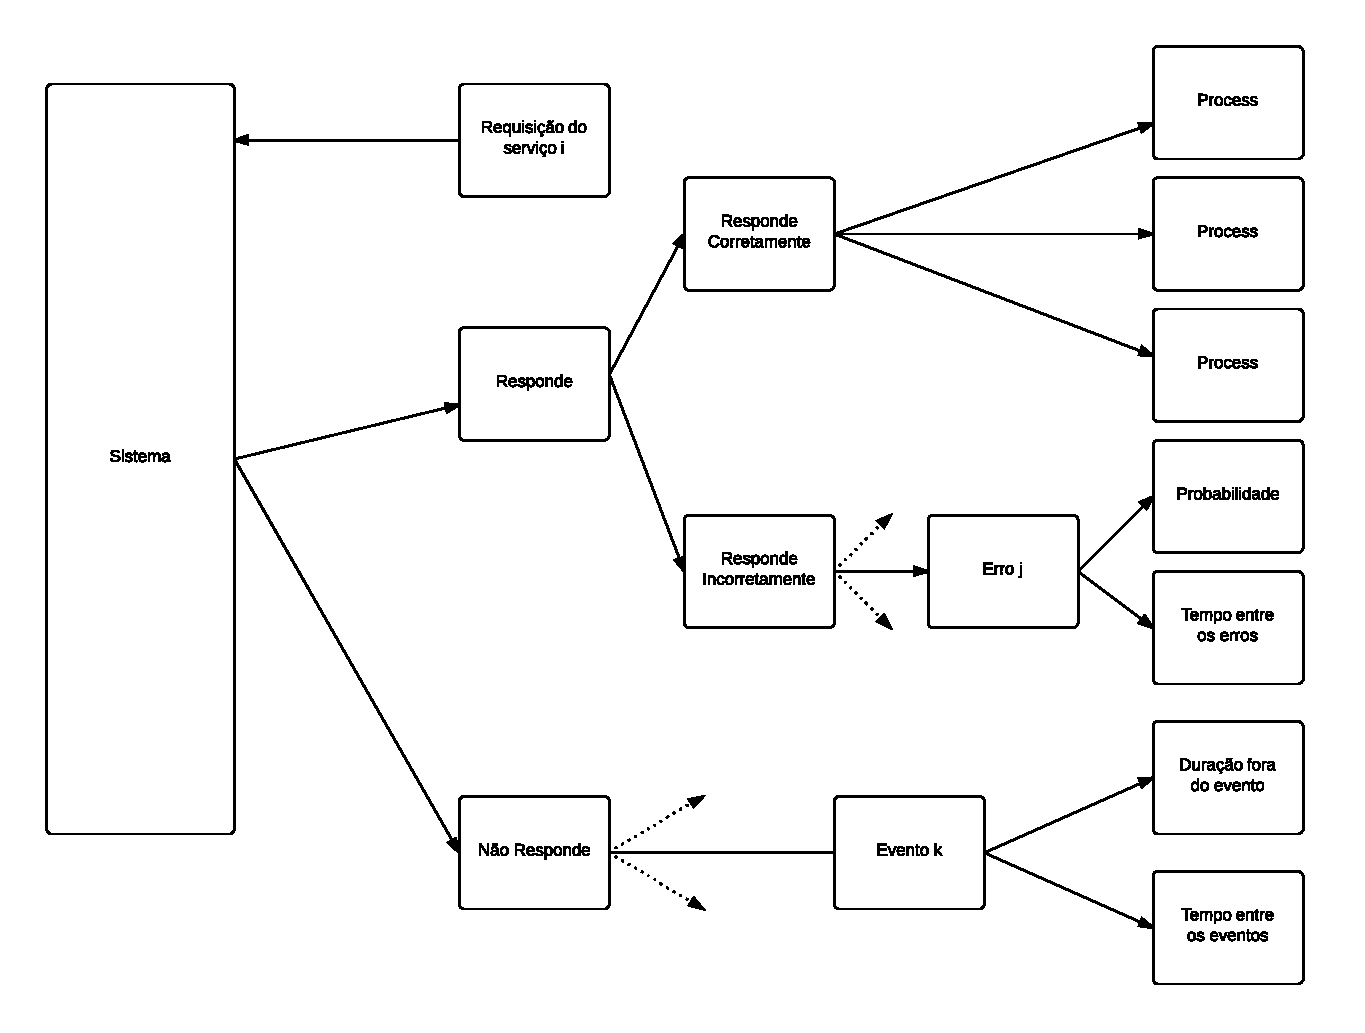
\includegraphics[scale=0.65]{imagens/saidarequisicao.pdf}
    \caption{Três possíveis resultados para requisições de serviços} \cite[p. 33]{Jain}
    \end{figure}

\section{Métricas de Desempenho Comumente Utilizadas}
\label{sec:metricas}
    
   Existem 3 métricas de desempenho mais comumente utilizadas, porém estas definições podem variar de acordo com o projeto \cite{Jain}. São elas:
    \begin{itemize}
    \item Tempo de Resposta: é definido como o intervalo entre a requisição do usuário e a resposta do sistema;
    \item Capacidade: relaciona a capacidade de processamento (requisições por unidade de tempo)  com o tempo de resposta do sistema e
    \item Eficiência: é a eficiência dos multi-processadores dos sistema. A razão entre o desempenho de um sistema \textit{n-processador} de um sistema \textit{one-processador} é a sua eficiência. O desempenho é geralmente medido em termos de MIPS ou MFLOPS.
    \end{itemize}